\documentclass[12pt,a4paper]{article}
\usepackage[left=15mm,right=15mm,top=14mm,bottom=19mm,footskip=9mm]{geometry}
\usepackage{iftex}
\ifPDFTeX
  \usepackage[T5]{fontenc}
  \usepackage[utf8]{inputenc}
  \usepackage{mathptmx}
\else
  \usepackage{fontspec}
  \IfFontExistsTF{Times New Roman}{\setmainfont{Times New Roman}}{\setmainfont{Tinos}}
\fi
\usepackage{amsmath,amssymb}
\usepackage{tikz}
\usetikzlibrary{arrows.meta}
\usepackage[most]{tcolorbox}
\usepackage{fancyhdr,lastpage}
\usepackage{tabularx,array}
\definecolor{sectionpurple}{RGB}{155,42,143}
\definecolor{notebackground}{RGB}{229,240,245}
\definecolor{noteborder}{RGB}{255,55,55}
\definecolor{graphred}{RGB}{188,55,61}
\definecolor{graphblue}{RGB}{45,95,200}
\setlength{\parindent}{0pt}
\setlength{\parskip}{2pt}
\setlength{\headheight}{15pt}
\setlength{\abovedisplayskip}{5pt}
\setlength{\belowdisplayskip}{5pt}
\setlength{\abovedisplayshortskip}{3pt}
\setlength{\belowdisplayshortskip}{3pt}
\pagestyle{fancy}
\fancyhf{}
\renewcommand{\headrulewidth}{0pt}
\renewcommand{\footrulewidth}{0.4pt}
\fancyfoot[L]{\fontsize{8.5}{10}\selectfont Tài liệu tổng hợp theo TDMXX09--TDMXX11 (Tư Duy Mở)}
\fancyfoot[R]{\fontsize{8.5}{10}\selectfont Trang \thepage/\pageref{LastPage} -- Bài giảng 05}
\newtcolorbox{notebox}{colback=notebackground,colframe=noteborder,
  boxrule=0.8pt,arc=2pt,left=7pt,right=7pt,top=3pt,bottom=3pt,
  before skip=3pt,after skip=3pt}
\newcommand{\partheading}[1]{\par\vspace{5pt}\noindent\textbf{\textcolor{sectionpurple}{#1}}\par\vspace{1pt}}
\newcommand{\example}[2][TDM21]{\par\vspace{3pt}\noindent\textbf{\textcolor{sectionpurple}{Ví dụ #2:} \textcolor{noteborder}{[#1]}}\enspace}
\newcommand{\tightitem}{\setlength{\itemsep}{1pt}\setlength{\topsep}{1pt}\setlength{\parsep}{0pt}\setlength{\partopsep}{0pt}}
\begin{document}
\fontsize{12}{14.6}\selectfont
\begin{center}
  \textbf{BÀI GIẢNG 05}\\[-1pt]
  \textbf{TIỆM CẬN XIÊN -- KHẢO SÁT VÀ VẼ ĐỒ THỊ HÀM SỐ}\\[-2pt]
  {\fontsize{10.5}{12}\selectfont\itshape Tổng hợp nội dung từ TDMXX09, TDMXX10 và TDMXX11}
\end{center}
\vspace{-7pt}

\partheading{PHẦN I. CƠ BẢN VỀ TIỆM CẬN XIÊN CỦA ĐỒ THỊ HÀM SỐ}
\example{1} Cho hàm số $y=f(x)$ có đồ thị $(C)$ và đường thẳng $d$ có phương trình $y=ax+b$ ($a\ne0$) như hình vẽ. Gọi $M,N$ là hai điểm có cùng hoành độ, lần lượt thuộc $(C)$ và $d$. Hãy xác định độ dài đoạn $MN$ khi $x\to+\infty$ ở hình (1), và khi $x\to-\infty$ ở hình (2).
\begin{notebox}
\centering
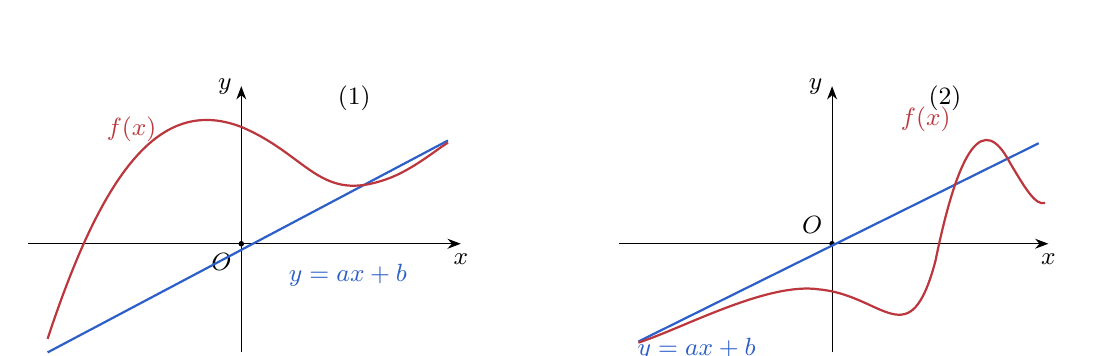
\begin{tikzpicture}[x=0.82cm,y=0.69cm,>=Stealth,every node/.style={font=\small}]
  % Panel 1: a line approached at positive infinity
  \begin{scope}[shift={(0,0)}]
  \draw[->,thin] (-3.3,0)--(3.4,0) node[below]{$x$};
  \draw[->,thin] (0,-2.0)--(0,2.9) node[left]{$y$};
  \fill (0,0) circle (1pt) node[below left]{$O$};
  \draw[graphblue,thick] (-3,-2)--(3.2,1.9);
  \draw[graphred,thick] (-3,-1.75) .. controls (-2.1,1.5) and (-1.2,2.7) .. (0,2.15)
    .. controls (1.0,1.65) and (1.2,0.8) .. (2.15,1.15)
    .. controls (2.6,1.3) and (3,1.72) .. (3.2,1.86);
  \node[graphred] at (-1.7,2.1) {$f(x)$};
  \node[graphblue,below] at (1.65,-0.2) {$y=ax+b$};
  \node at (1.75,2.67){(1)};
  \end{scope}
  % Panel 2: a line approached at negative infinity
  \begin{scope}[shift={(9.15,0)}]
  \draw[->,thin] (-3.3,0)--(3.35,0) node[below]{$x$};
  \draw[->,thin] (0,-2.0)--(0,2.9) node[left]{$y$};
  \fill (0,0) circle (1pt) node[above left]{$O$};
  \draw[graphblue,thick] (-3,-1.8)--(3.2,1.85);
  \draw[graphred,thick] (-3,-1.82) .. controls (-2.3,-1.55) and (-1.0,-0.70) .. (-0.2,-0.84)
    .. controls (0.8,-0.95) and (1.2,-2.1) .. (1.6,-0.32)
    .. controls (1.97,1.83) and (2.35,2.4) .. (2.75,1.5)
    .. controls (3.0,1.0) and (3.15,0.7) .. (3.3,0.75);
  \node[graphred] at (1.45,2.3) {$f(x)$};
  \node[graphblue,below] at (-2.1,-1.55) {$y=ax+b$};
  \node at (1.75,2.67){(2)};
  \end{scope}
\end{tikzpicture}
\end{notebox}
\textbf{Định nghĩa.} Đường thẳng $y=ax+b$ ($a\ne0$) được gọi là \textbf{tiệm cận xiên} của đồ thị $y=f(x)$ nếu
\[
  \lim_{x\to+\infty}\bigl[f(x)-(ax+b)\bigr]=0
  \quad\text{hoặc}\quad
  \lim_{x\to-\infty}\bigl[f(x)-(ax+b)\bigr]=0.
\]
\textbf{Nhận xét.}
\begin{enumerate}\tightitem
  \item Đồ thị hàm số có tiệm cận xiên thì tập xác định của hàm số phải chứa ít nhất một khoảng vô cực.
  \item Tiệm cận xiên có thể không có, có một hoặc có nhiều điểm chung với đồ thị $(C)$.
  \item Một đồ thị có tối đa hai tiệm cận xiên (ứng với hai phía $+\infty$ và $-\infty$); cũng có thể chỉ có một hoặc không có tiệm cận xiên.
\end{enumerate}
\textbf{Cách tìm phương trình tiệm cận xiên.} Xét riêng mỗi phía vô cực:
\[
\begin{aligned}
 x\to+\infty:&\quad a=\lim_{x\to+\infty}\frac{f(x)}{x},\qquad
 b=\lim_{x\to+\infty}\bigl[f(x)-ax\bigr];\\
 x\to-\infty:&\quad a=\lim_{x\to-\infty}\frac{f(x)}{x},\qquad
 b=\lim_{x\to-\infty}\bigl[f(x)-ax\bigr].
\end{aligned}
\]
Các giới hạn trên cần hữu hạn và $a\ne0$. Nếu $a=0$ và $\lim f(x)=b$ hữu hạn tại phía đang xét thì đường thẳng $y=b$ là \textbf{tiệm cận ngang}, không phải tiệm cận xiên.
\begin{notebox}
\example[TDM31]{2} Hãy xác định tiệm cận xiên của đồ thị các hàm số sau:
\begin{enumerate}\tightitem
\item $y=f(x)=\dfrac{x^2-4x+5}{x-1}$.
\item $y=g(x)=\sqrt{4x^2+2x+1}-x$.
\end{enumerate}
\end{notebox}

\partheading{PHẦN II. KHẢO SÁT HÀM SỐ BẬC BA}
\textbf{Sơ đồ khảo sát sự biến thiên và vẽ đồ thị của hàm số:}
\begin{enumerate}\tightitem
\item \textbf{Tập xác định.}
\item \textbf{Sự biến thiên:} Tìm các giới hạn tại vô cực, giới hạn vô cực và các đường tiệm cận (nếu có); tính đạo hàm, xét dấu đạo hàm, xét chiều biến thiên, tìm cực trị và lập bảng biến thiên.
\item \textbf{Đồ thị:} Vẽ các đường tiệm cận (nếu có); xác định điểm đặc biệt (điểm cực trị, giao với trục tọa độ trong trường hợp đơn giản,\ldots); nhận xét tâm đối xứng, trục đối xứng (nếu có).
\end{enumerate}
\begin{notebox}
\example{1} Khảo sát sự biến thiên và vẽ đồ thị của hàm số $y=x^3-3x+2$.
\end{notebox}
\begin{notebox}
\example{2} Khảo sát sự biến thiên và vẽ đồ thị của hàm số $y=-x^3+3x^2-4x+4$.
\end{notebox}
\textbf{Các dạng đồ thị hàm bậc ba $y=ax^3+bx^2+cx+d$ ($a\ne0$):}
\begin{notebox}
\centering
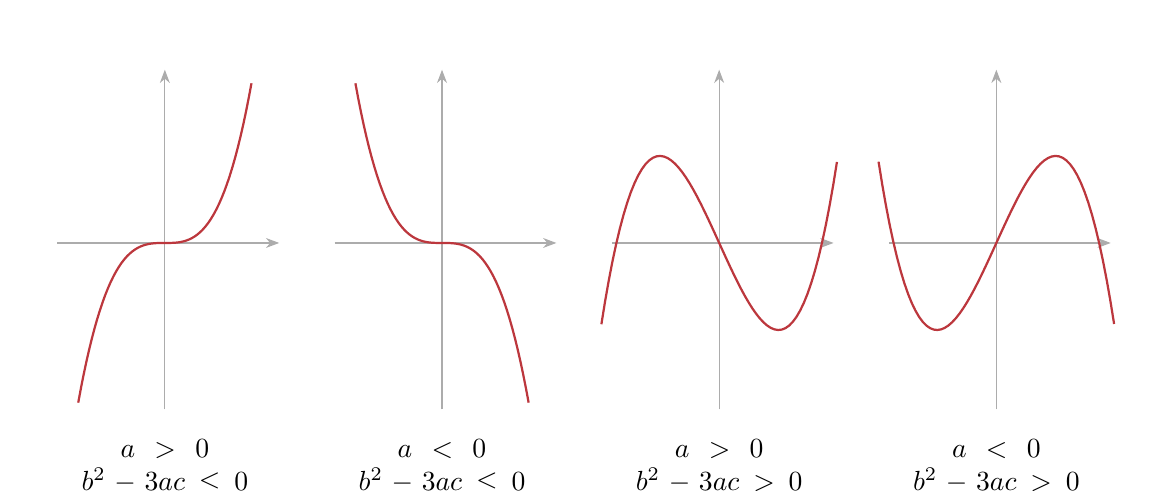
\begin{tikzpicture}[>=Stealth,scale=0.88]
  \begin{scope}[shift={(0,0)}]
    \draw[gray!65,->] (-1.55,0)--(1.65,0); \draw[gray!65,->] (0,-2.4)--(0,2.5);
    \draw[graphred,thick,domain=-1.25:1.25,samples=65] plot (\x,{1.18*\x*\x*\x});
    \node[align=center,text width=3.25cm,anchor=north] at (0,-2.7) {$a>0$\\$b^2-3ac\leq0$};
  \end{scope}
  \begin{scope}[shift={(4.0,0)}]
    \draw[gray!65,->] (-1.55,0)--(1.65,0); \draw[gray!65,->] (0,-2.4)--(0,2.5);
    \draw[graphred,thick,domain=-1.25:1.25,samples=65] plot (\x,{-1.18*\x*\x*\x});
    \node[align=center,text width=3.25cm,anchor=north] at (0,-2.7) {$a<0$\\$b^2-3ac\leq0$};
  \end{scope}
  \begin{scope}[shift={(8.0,0)}]
    \draw[gray!65,->] (-1.55,0)--(1.65,0); \draw[gray!65,->] (0,-2.4)--(0,2.5);
    \draw[graphred,thick,domain=-1.7:1.7,samples=65] plot (\x,{\x*\x*\x-2.2*\x});
    \node[align=center,text width=3.25cm,anchor=north] at (0,-2.7) {$a>0$\\$b^2-3ac>0$};
  \end{scope}
  \begin{scope}[shift={(12.0,0)}]
    \draw[gray!65,->] (-1.55,0)--(1.65,0); \draw[gray!65,->] (0,-2.4)--(0,2.5);
    \draw[graphred,thick,domain=-1.7:1.7,samples=65] plot (\x,{-\x*\x*\x+2.2*\x});
    \node[align=center,text width=3.25cm,anchor=north] at (0,-2.7) {$a<0$\\$b^2-3ac>0$};
  \end{scope}
\end{tikzpicture}
\end{notebox}

\partheading{PHẦN III. KHẢO SÁT VÀ VẼ ĐỒ THỊ HÀM PHÂN THỨC}
\textbf{1. Dạng phân thức bậc nhất trên bậc nhất:}
\[
  y=\frac{ax+b}{cx+d},\qquad c\ne0,\quad ad-bc\ne0.
\]
\begin{notebox}
\example{1} Khảo sát sự biến thiên và vẽ đồ thị của hàm số $y=\dfrac{x+2}{x-1}$.
\end{notebox}
\textbf{2. Dạng phân thức bậc hai trên bậc nhất:}
\[
  y=\frac{ax^2+bx+c}{mx+n},\quad a,m\ne0,\quad
  a\left(-\frac{n}{m}\right)^2+b\left(-\frac{n}{m}\right)+c\ne0.
\]
\begin{notebox}
\example{1} Khảo sát sự biến thiên và vẽ đồ thị của hàm số $y=\dfrac{x^2-4x+5}{x-2}$.
\end{notebox}
\begin{notebox}
\example{2} Khảo sát sự biến thiên và vẽ đồ thị của hàm số $y=\dfrac{x^2-2x-3}{x-1}$.
\end{notebox}
\vspace{1pt}
{\centering\textbf{\textcolor{sectionpurple}{--- Hết ---}}\par}
\end{document}